% Tesis ITAM CLASS -- version 0.1 (13 - Abr - 2015)
% Clase para las tesis del ITAM
%
% 13 - Abr - 2015 	Victor Martinez 	victor.martinez (at) itam.mx
% LICENSE: Creative Commons SA-BY 3.0
%
%
% Este documento presenta un ejemplo de uso de la plantilla
% El estudiante es libre de modificar este archivo a su gusto
%
\documentclass{tesisITAM}
\usepackage[utf8]{inputenc}
\usepackage{amsmath}
\usepackage{comment}
\usepackage{multirow}
\usepackage{hyperref}
%\usepackage{cite}
%\usepackage[]{apacite}
%\usepackage{natbib}


%\usepackage{csquotes}
%\usepackage[style=apa]{biblatex}


\title{Creatividad artificial: imitación de estilos musicales}
\author{Emir Herrera González}
\degree{Ing. en Telemática}
\advisor{Andrés Gómez de Silva}
\year{2015}

\begin{document}

	\pagenumbering{gobble}
	\maketitle
	\publicationrights

	%%%%%%%%%%%%%%%%%%%%%%%%%%%%%%%%%%%%%%%%%%%%%%
	% ABSTRACT
	%%%%%%%%%%%%%%%%%%%%%%%%%%%%%%%%%%%%%%%%%%%%%%

	\begin{abstract}{spanish}
	\end{abstract}

	\begin{abstract}{english}
	\end{abstract}


	\selectlanguage{spanish}
	\setcounter{page}{1}
	\pagenumbering{roman}

	\tableofcontents
	\listoffigures
	\listoftables
	\newpage

	\pagenumbering{arabic}
	\setcounter{page}{1}

	%%%%%%%%%%%%%%%%%%%%%%%%%%%%%%%%%%%%%%%%%%%%%%
	% CONTENT
	%%%%%%%%%%%%%%%%%%%%%%%%%%%%%%%%%%%%%%%%%%%%%%

		\chapter{Análisis del problema}
			\label{ch:analisis}

			\chapter{Introducción}
\begin{comment}

Aparte de que faltarían muchos capítulos, en las partes que escribiste hay mucho “qué” (es decir, explicaciones de lo que se hizo), pero falta mucho “por qué” (explicaciones/justificaciones de por qué se hizo, y de por qué se hizo de la manera en la que se hizo y no de cualquier otra manera).

¿Puede una computadora crear algo útil para el ser humano con un universo de elementos previamente provistos por el humano?.
Las tragedias griegas originalmente iban representadas con canto y danza, y se consideraba la poesía, la musica y la danza un solo arte.

¿Cómo surge el sentido de la belleza en el ser humano?

\end{comment}

\begin{comment}
\section{sin nombre}

Una computadora es probablemente la herramienta más útil con la que cuenta el ser humano hoy día, nos ha permitido ir a la luna, mejorar nuestros sistemas de comunicaciones, crear prótesis biónicas

En la actualidad existe una especie de simbiosis humano-máquina cómo probablemente no ha existido en la historia entre el humano y otro ser vivo, al menos de forma conciente. Si bien el ser humano se ha beneficiado mucho de las máquinas no podemos decir que una máquina se haya beneficiado de un humano, responder si una actualización de software o hardware significa un beneficio para la máquina está fuera del proposito de este trabajo, sin embargo asumiremos como premisa el hecho de que una computadora carece de conciencia y que el beneficio o perjucio sólo existen en seres concientes.

\end{comment}

\section{¿Qué es la creatividad?}
\paragraph{Se entiende como creatividad la facultad de crear algo novedoso, ideas, conceptos u objetos tangibles que tengan alguna utilidad. Esta caracteristica de utilidad es lo que diferencia una idea creativa de una tonta.}

\section{¿Qué es la creatividad artificial?}
\paragraph{La Creatividad Artificial es un esfuerzo multidisciplinario en el que intervienen distintas áreas tales como Inteligencia Artificial, Filofosía, Ciencias Cognitivas y Artes. El objetivo es crear un software que replique la creatividad tal cómo esta ocurre en el nivel humano.}

\section{Objetivo}
\paragraph{En esta tesis se analizan las caracteristicas de una obra musical, se plantea la posibilidad de que una computadora cree una obra musical que comparta carácteristicas sonoras con otras obras previas de un mismo artista. Partiendo del hecho de que una obra puede ser atribuida a un artista por su estilo se describe un modelo probabilistico del estilo y mediante el uso de Algoritmos Genéticos se desea crear una obra que comparta las características de ese estilo.}

\paragraph{La presente tesis aborda el proceso creativo cómo combinación de elementos existentes en el entorno con la finalidad de crear algo que no existía antes en el entorno. Hasta la fecha no existe un modelo que replique a la perfección el proceso creativo de un humano.}

\paragraph{Entendemos cómo creatividad la facultada de generar nuevas ideas o conceptos.}

\paragraph{Se entiende cómo proceso creativo creatividad la mezcla de memorias, combinadas de forma coherente, cuya expresión es novedosa y tiene significado dentro de un contexto colectivo especifico, cuando la interpretación de esta expresión de memorias es incomprencible por agentes externos dentro del mismo contexto, se dice que la idea es incoherente.}

\paragraph{La creatividad y el arte son resultado de cómo el cerebro humano opera con los datos percibidos por los organos sensoriales. Podemos reconocer momentos creativos en sueños, mientras estamos absortos en algún pensamiento concreto o cuanto "de la nada" nos llega una idea aperentemente sin relación con la actvidad actual.}

\paragraph{Algún tipo cuyo nombre y obra no recuerdo\cite{required} distingue entre creatividad psicológica y creatividad histórica, en dónde la creatividad histórica es aquella idea nueva que nunca se ha hecho antes y la creatividad psicólogica es aquello nuevo en la mente del individuo.}


\paragraph{El presente proyecto pretende imitar el estilo musical de un autor, mediente el uso de algoritmos genéticos se pretende generar una nueva pieza musical que sea lo más parecida a un estilo musical determinado.}

			\section{Objetivo}

Necesito una nueva pieza musical de [Inserte autor aquí], ¿qué debo hacer?" (EdwardBono)
El presente proyecto pretende imitar el estilo musical de un autor, mediente el uso de algoritmos genéticos se pretende generar una nueva pieza musical que sea lo más parecida a un estilo musical determinado.
Se pretende generar una melodía en formato MIDI que comparta características estéticas del estilo de Francisco Tarrega sin que sea confundible con una composición previamente conocida del mismo autor.

Desarrollar un sistema autonomo capaz de componer una pieza musical muy similar al estilo de un compositor especifico.

Es posible crear una pieza musical similar a otras piezas musicales de un autor determinado realizando combinaciones aleatorias en las notas musicales y conservando aquellos conjuntos de notas cuyo arreglo se asemeje en la mayor medida posible sobre la combinación de notas que posiblemente hubiera realizado el autor o estilo que se quiere imitar.

%	\section{Definición del problema}
%
%	\section{Alcance}

%		\item ¿Que elementos tienen en común el estilo y el genero?
%		\item ¿Cómo se define matematicamenet el dominio de la música?
%		\item ¿Puede diferenciarse el estilo musical si todas las notas se tocan en la misma octava?
%
%		\item ¿Qué es un beat?
%			Un beat mide en segundos la duración de la figura musical (tambien llamada nota) de menor valor en una pieza musical.
%
%		\item ¿Qué es la creatividad humana?
%				Es la facultad que tiene el humano de crear
%				La creatividad humana se conoce cuando se entra en contacto con ella, debe ser novedoso y entendible.
%

			\section {Arte}

\paragraph{
  "La obra es el origen del artista. Ninguno puede ser sin el otro. Pero ninguno de los dos soporta tampoco al otro por separado. El artista y la obra son en sí mismos y recíprocamente por medio de un tercero que viene a ser lo primero, aquello de donde el artista y la obra de arte reciben sus nombres: el arte" \cite{heidegger-1936}.
}

\paragraph{
  Para que algo sea considerado arte debe existir una apreciación subjectiva que le valorice cómo tal.
}

\paragraph{
  Al arte aunque se trate de una existencia efímera, existe en el mundo material y cómo tál está conformado por una configuración particular de elementos únicos y finitos.
}

\paragraph{
  El arte tiene la particularidad de cada reconfiguración de sus elementos en un instante determinado y/o su transición a la siguiente configuración reasemeja sensaciones conocidas al expectador.
}

\paragraph{
  Si consideremaos que \it{la inspiración} produce de una reconfiguración de elementos previamente conocidos, una creación que surge de la nada es [primer motor]
}


\section{Música}

\paragraph{
  La música es una forma de expresión creada por el ser humano, mediante sonidos intercalados ensambla armonias.
  El silencio sólo existe cómo idea abstracta o en aquellos espacios en los que el sonido no puede viajar, e incluso cuando el sonido no viaja existen objetos que vibran en frecuencias audibles. Un espacio completamente en silencio ha carecer incluso de observador.
}

			\section{Antecedentes}
- Creatividad artificial
- Imitación computarizada

			\section{El formato MIDI}
	El formato MIDI permite representar en forma digital las notas tocadas por un instrumento musical en forma de eventos. El un MIDI puede representar hasta 16 canales, cada uno asociado a un instrumento. Cuando un instrumento sólo puede producir una sola nota, se dice que es un instrumentono monótono

\begin{verbatim}
>> [max(tarreaga);min(tarreaga);max(tarreaga)-min(tarreaga)]

ans =

	379.6250    3.0000    2.0000   88.0000  100.0000  197.5583    1.9167
				 0    0.1250    1.0000   40.0000  100.0000         0    0.0625
	379.6250    2.8750    1.0000   48.0000         0  197.5583    1.8542
\end{verbatim}

\section {Conteo del dominio del problema}
  Definir el dominio del problema (espacio musical)
    ¿Cuantas posibilidades existen para componer una melodía?

    Las posibilidades de la música extrictamente hablando son infinitas, sin embargo podemos acotar el dominio acotando su extensión temporal y la cantidad de notas a elegir

    ¿Cuántos beats existen en una grabación de duración T?
      Si un beat tiene una duración t,

		El número de beats n se obtiene mediante la fórmula \eqref{eq:n}

			\begin{equation} \label{eq:n}
				n = \frac{T}{t}
			\end{equation}


		%		1. Análisis del problema
		%			* Hipótesis
		%			  * Una computadora puede mostrar carácteristicas creativas.
		%			  * Una computadora es capaz de generar una melodía utilizando algoritmos genéticos.
		%			* Objetivo
		%			* Marco teórico
		%		2. Investigación
    \chapter{Composición musical}
    \section{Figura Musical}

        \paragraph{Una figura en el pentagrama, represneta la nota, su posición y duración temporal. Es posible entonces representar a cada nota musical cómo un objeto con tres propiedades escenciales, su frecuencia, el momento de inicio y el fomento final.}

        \paragraph{Un gen que mutó recientemente tiene menos posibilidades de ser elegido para la siguiente mutación. Los puntos de cruce serán escogidos con base al fitness de cada individuo, el individuo con mayor fitness le heradará los genes predominantes a la siguiente generación.}

        \subsection{Cruces}
          \paragraph{El punto de cruce se elige en función de una distribución normal cuya media es el resultado de la función fitness, normalizado, de el primer fenotipo}

          \begin{equation}
              \mu = \frac{fitness(fenotipo_1)}{fitness(fenotipo_1) + fitness(fenotipo_2)}
          \end{equation}
          \begin{equation}
              CP \sim N(\mu,1)
          \end{equation}

          \paragraph{El primer fenotipo será el que aporte los genes a la izquierda. El nuevo genotipo resulta de cortar en la fracción CP a los dos fenotipos, y uniendo el lado izquiero del $fenotipo_{1}$ con la parte derecha del $fenotipo_{2}$. El gen intermedio, el que corresponde al punto de corte se recalcula, promediando los valors de ambos fenotipos para el valor de la nota y suduración, la posición temporal es la que correspondé al $fenotipo_{1}$. Las posiciones temporales del $fenotipo_{2}$ se recalculan antes de aderir los genes al nuevo fenotipo siguiendo la formula:}

          \begin{equation}
              \overline{T} = \overline{T_{2}}  - min(\overline{T_{2}}) + max(\overline{T_{1}})
          \end{equation}

    \section {Armonia}
    \section {Definición del estílo}
    \section {Contorno melódico}

    \chapter{Creatividad}
\section{Definicion}
\paragraph{La RAE define creatividad como {\it facultad de creación}}

\paragraph{En el sentido estricto, resulta imposible crear algo de la nada, a lo más podemos trabajar con elementos basicos ya existentes y crear un ensable nuevo de esos elementos, al conjunto resultante, cuandpor la ley de la conservación de la energía, se puede decir que es imposible conocer el proceso creativo mediante el cuál algo surge de la nada. Lo que socialmente conocemos como creatividad humana, es un proceso de razonamiento mediante el cuál un ser humano reconfigura ediante un conjunto de pensamientos elementos prexistentes para darle forma a algo que antes no existía y que tiene un valor social, si el objeto nuevo sólo es apreciable por su creador no es considerado resulado de un proceso creativo.}

\paragraph{Todo trabajo creativo humano es resultado de un trabajo anterior, la música por ejemplo, no existiría si no hubiera un instrumento, el instrumento no produciría sonido si no existiera un material con que moldearlo, el material no seria moldeable si sus atomos no tuvieran determinada configuración, etcétera.}

\paragraph{Vemos que existe una energía fínita en el universo con posibilidades (una n muy grande) infinitas de configuración; entre la luz y la materia sólida existe un espectro finito extremadamente amplio. De esta observación concluimos que la creatividad humana se lleva a cabo dentro de un dominio material finito, con posibilidades incuantificables, pero con una apreciación limitada por el entorno social, no toda combinación tiene un significado para el entorno.}

\paragraph{La música es un arreglo de frecuencias sonoras estandarizadas, cuyo orden y duración producen una pieza musical, definimos el dominio de la música al conjunto de notas musicales reproducibles en un instrumento musical. La diferencia entre la música y el ruido es que el ruido carece de significado, un instrumento musical desafinado puede producir sonidos molestos para el oyente. Lo que para un artísta podría ser una obra maestra, si no transmite al receptor algo con significado no es producto de la creatividad.}

\section{Creatividad Artificial}

El dominio en el que existe la creatividad


Existen muchas deficiones de creatividad, la RAE la define cómo la capacidad de creación, si pensamos ue todo lo que crea el hombre existe ya dentro de un dominio finito


La creatividad la reconocemos por su resultado

\section{Tipos de creatividad}

\paragraph{Existen dos tipos de creatividad, la creatividad histórica y la creatividad psicológica\cite{pensamiento-creativo} }
\paragraph{Algún tipo cuyo nombre y obra no recuerdo  distingue entre creatividad psicológica y creatividad histórica, en dónde la creatividad histórica es aquella idea nueva que nunca se ha hecho antes y la creatividad psicólogica es aquello nuevo en la mente del individuo.}


\begin{comment}
    De existir una máquina capaz de analizar el lenguaje humano, e.i. operar con todo el conocimiento humano disponible y los problemas humano, esa máquina sería capaz de proponer soluciones novedosas a los problemas humanos.

    ¿Es posible crear una máquina que invente un avión a partir de las leyes de la física y el requisito: volar?
\end{comment}


\section {Psicología de la creatividad}
\paragraph {No existe una defición concreta de creatividad, sin embargo todos los intentos por definir la creativid coinciden en que el resultado de la creatividad es la producción de algo que no existia previamente, pero tambien hay un factor social, no todas las creaciones novedosas son creativas, vemos que es necesario el reconocimiento de algún tercero para que la creación sea considerada creativa.}

\paragraph {Consideramos que la creatividad es una expresión de la originalidad de cada individuo, es poco probable que dos individuos creen una copia identica del mismo trabajo cuando se les deja actuar libremente a merced de su imaginación, la imaginación juega un papel importante en la creatividad, es ahi donde se producen ideas nuevas, aunque no todas puedan ser realizables, interviene tambien la inteligencia para poder dicernir lo realizable de las utopias.}

\paragraph {La creatividad de un sistema no se puede medir solamente con base en su salida, hay que tomar en consideración también la forma en la que el artefacto es producido. Entre los consumidores de arte ua obra es mejor valuada cuando el proceso mieante el que se hizo es más creativo. \cite{simon-colton}}

\section{Proceso creativo}

\paragraph{Habilidad, apreciación  e imaginación}
\section{Creatividad en la naturaleza}
\section{Creatividad artificial}


\section{Imitación de estilos}
  3. Codificar el fenotipo de una melodía
  4. Definir el proceso de mutación y cruce
  5. Definir el tamaño de la población
  6. Definir condificación de paro
    ¿Cuánto tiempo tomaría explorar el universo completo de posibilidades?

    Experimentos Set 2:
    1.- Generar un armónimo.
    2.- Generar una secuencia monótona
    3.- Generar una secuencia de armónicos.
    4.- Producir una secuencia monótona imitando un estílo musical
    5.- Producir una secuencia de armónicos imitando un estílo musical.


\section{Presentación}

  Autómata generador de melodías

  \paragraph{Los instrumentos musicales tienen una}
  \paragraph{Si consideramos una cantidad finita de generadores de }

    \chapter{Análisis melódico}
\section{Metodología}
\subsection{Análisis melódico}

\paragraph{Para el próposito de identificar la estructura común de un subconjunto de melodías, el estílo de un autor, y la asociacioón de una melodía en particular con un subconjunto dado con base en las similiaridades estructurales, empleamos}

\subsection{Wavelets}
\subsection{Modelo Oculto de Markov}
\subsection{Algoritmos Genéticos}

		%		3. Diseño de la solución
		%			* Desarrollo
		%			  * Metodología
		%			  * Experimentación
		%			  * Resultados
		\chapter {Implementación}
    \section {El dominio de las frecuencias}
    \section {Distribución de frecuencias}
    \section {Similitudes en la distribución de frecuencias}
    \section {Generación melódica}
    \section {Evolución creativa}



\section{Clasificación de melodías}


\subsection{Descripción del conjunto de entrenamiento}
\paragraph{La base de conocimiento cuenta con un total de 165 melodías, distribuidas de la siguiente forma:}


\input{draft/implementacion/knowledgebase.lst}

\subsection{Medición de la influencia entre compositores}
\paragraph{Para determinar si el sistema es capaz de identificar el compositor original de una melodía y que ta}

\begin{figure}[h]
    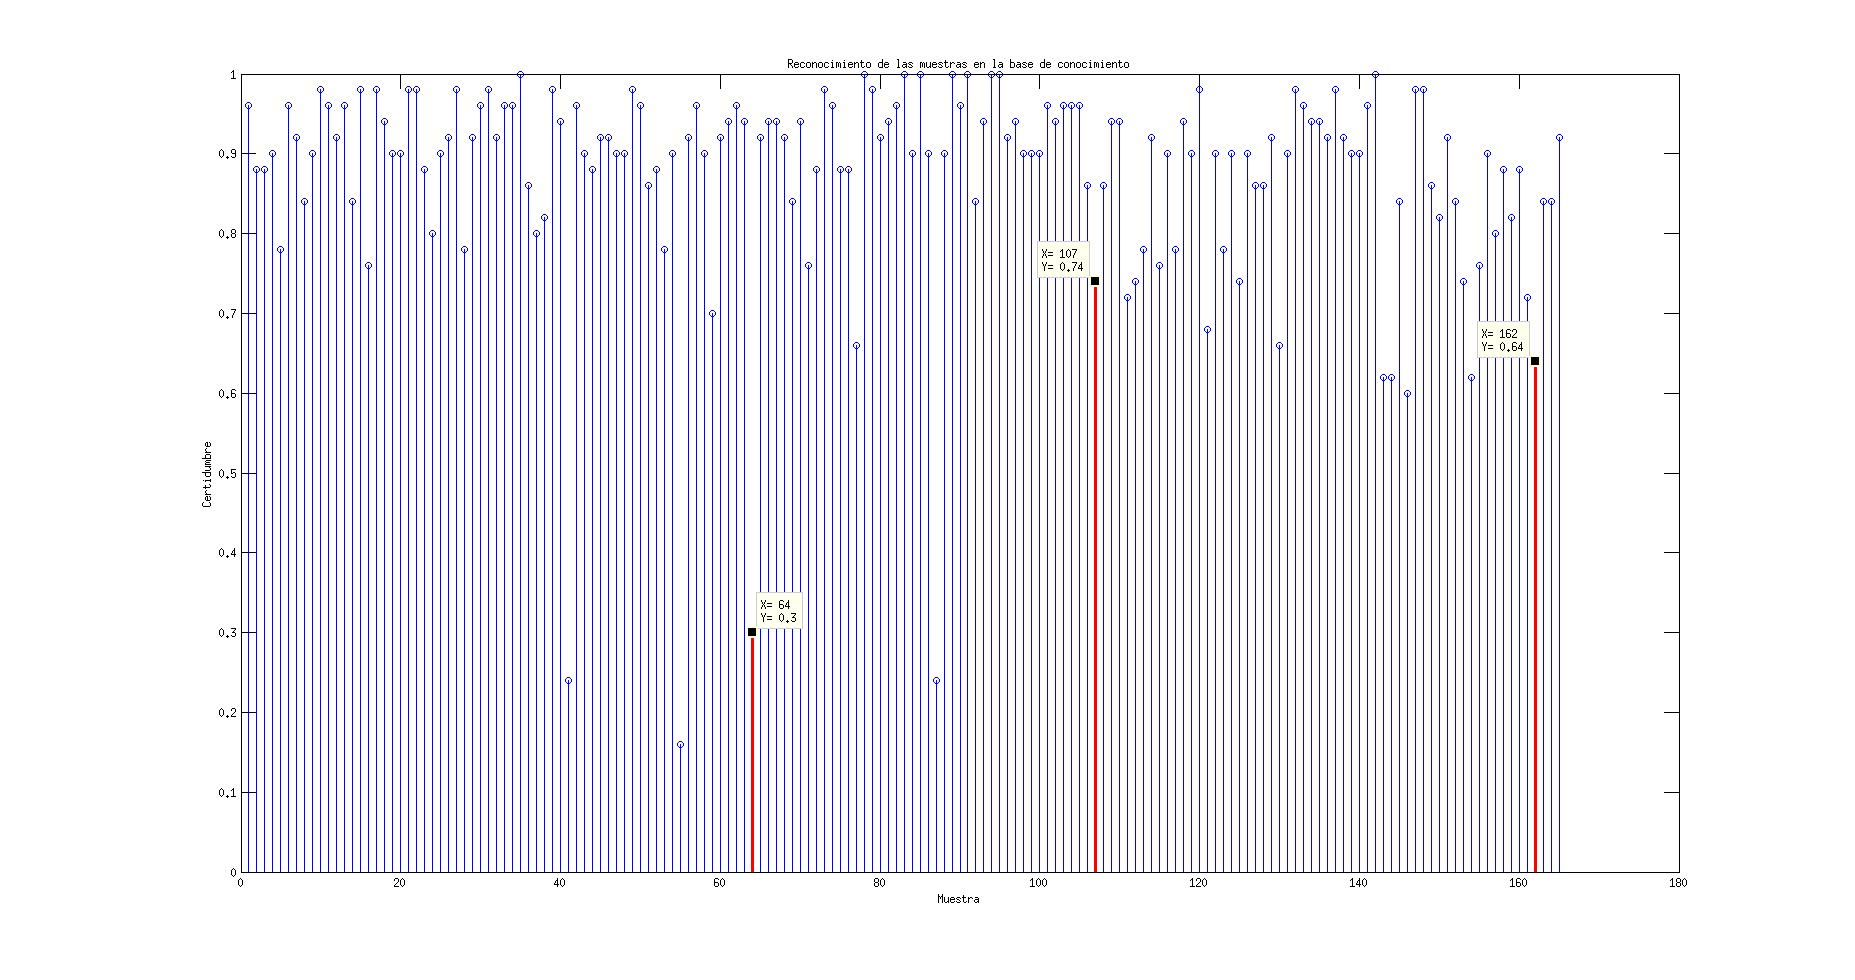
\includegraphics[width=0.9\textwidth]{draft/implementacion/img/covers_kbq.jpg}
    \caption{Certidumbre en el reconocimiento correcto de las melodías del conjunto de entrenamiento}
\end{figure}

\begin{figure}[h]
    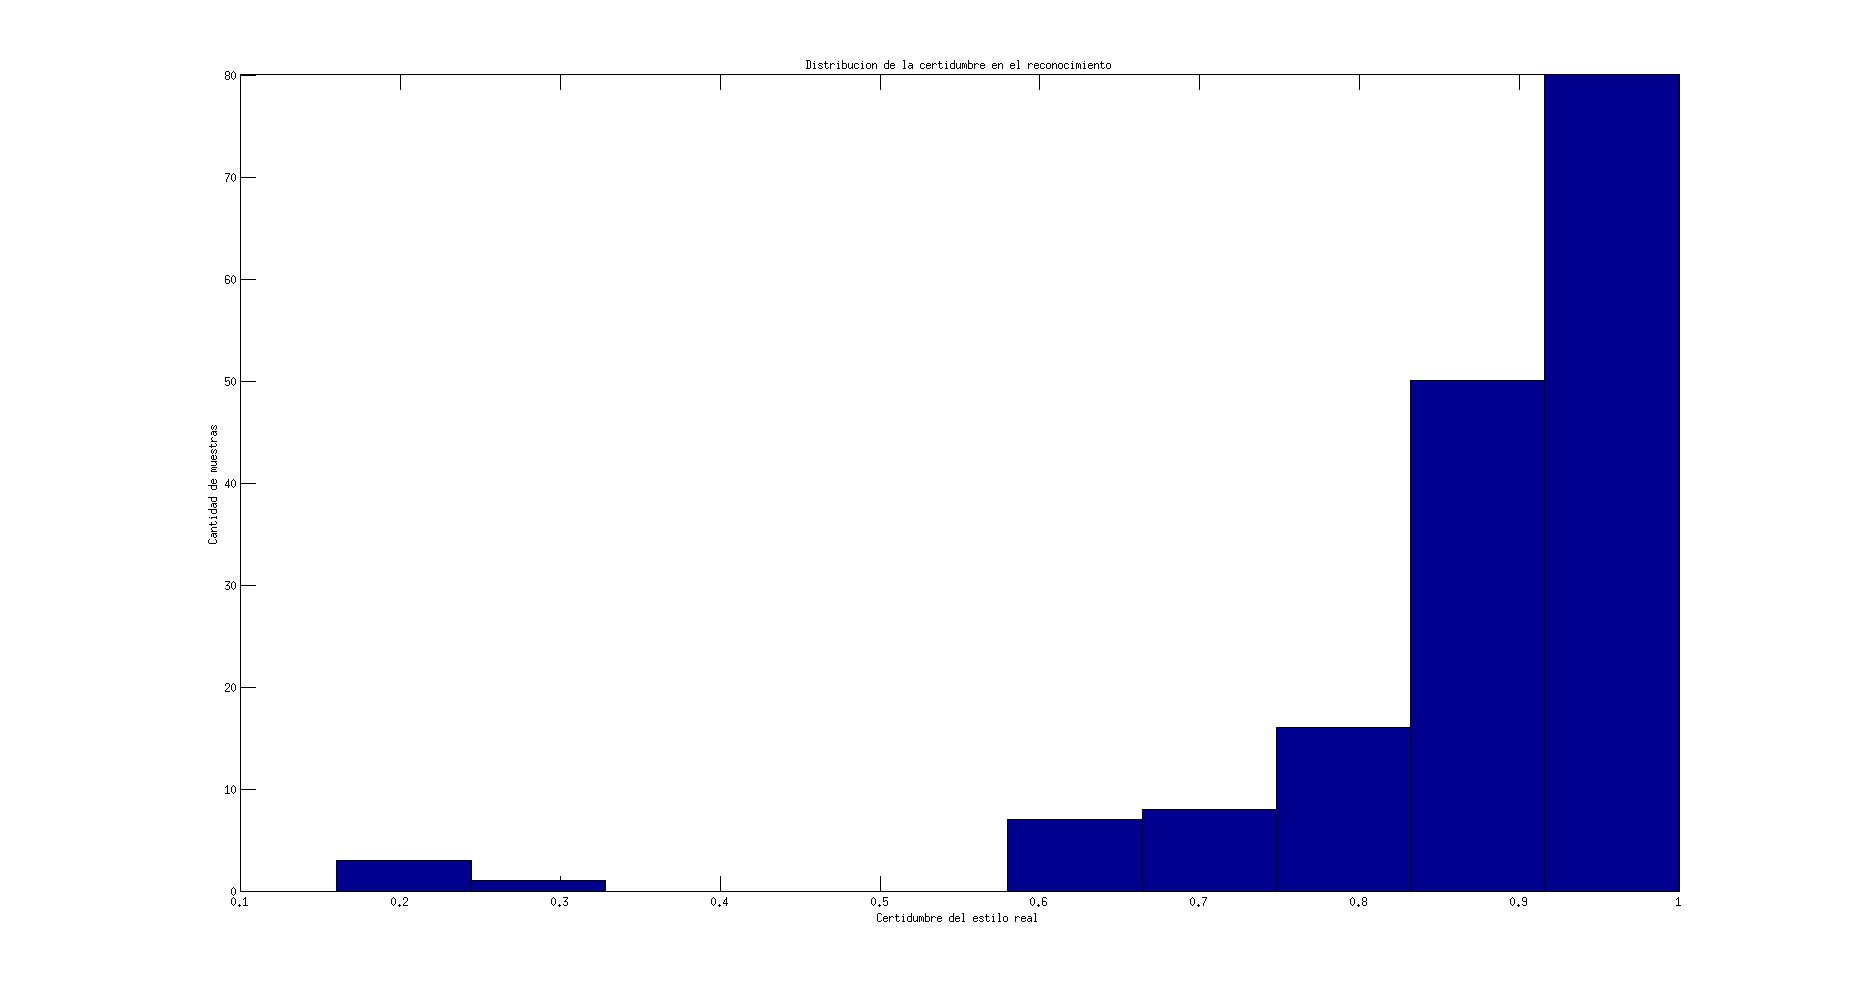
\includegraphics[width=0.9\textwidth]{draft/implementacion/img/fitness_histograma.jpg}
    \caption{Distribución de la certidumbre del conjunto de entrenamiento}
\end{figure}

\begin{center}
    \begin{tabular}{| c | c | c | c |}
        \hline
        \multirow{2}{*}{Interprete} & \multicolumn{3}{|c|}{Similitud media con} \\
         & Frank Sinatra & Elvis Presley & Sex Pistols \\ \hline
        Frank Sinatra & 40.66\% & 59.33\% & 0\% \\
        Elvis Presley & 2.66\% & 28\% & 69.33\% \\
        Sex Pistols & 77.33\% & 19.33\% & 3.33\% \\
        \hline
    \end{tabular}
\end{center}

\section{Reconocimiento de estilos}
  1. Definir el número de muestras a utilizar para entrenar el sistema
  2. Entrenar el sistema para que reconozca un estílo musical
    ¿Cuanto tiempo toma procesar una melodía?
    ¿Cuánto tiempo máximo podría tomar encontrar un resultado?

  Experimentos Set 1 Entrenamiento:
    1.- Identificación del interprete de una canción.
    2.- Identificación del autor de un cover.
    3.-

    \chapter{Resultados}
\section{Dudas durante el desarrollo}
\paragraph{Dado un conjunto de entrenamiento, ¿cuál es la melodía de menor duración con una clasificaión aceptable?, ¿cómo varia la tasa de certidumbre con la variación de la longitud de la melodía?, ¿que relación existe entre el tamaño de la Base de Conocimeinto y la certidumbre?, ¿y la entropía cómo se relaciona?}


\section {Eficiencia del entrenamiento}
\paragraph {Al momento de entrenar el sistema con diversos estílos musicales nos interesa que el sistema sea capaz de clasificar con un alto grado de confiabilidad diversas melodias, hay que tener en cuenta que al maximizar la confiabilidad tambien crece el tiempo requerido para procesar una pieza musical.}

\section {Eficiencia del sistema creativo}
\paragraph {En psicología una aproximación para medir la creatividad de una persona es el tiempo que le toma llegar a una solución original, siguiendo esta linea tomaremos como eficiencia del sistema el tiempo que le toma componer una pieza musical, empezando desde el momento en el que se entrena el sistema.}

\section {Evaluación humana de las composiciones}
        
		%		4. Análisis de los resultados
		%			* Conclusión




	% \input{Chapters/relatedwork}

	% \input{Chapters/method}

	% \input{Chapters/results}

	% \input{Chapters/conclusions}

	%%%%%%%%%%%%%%%%%%%%%%%%%%%%%%%%%%%%%%%%%%%%%%
	% APPENDIX
	%%%%%%%%%%%%%%%%%%%%%%%%%%%%%%%%%%%%%%%%%%%%%%
	\appendix
	% \input{Chapters/appendixA}

	%%%%%%%%%%%%%%%%%%%%%%%%%%%%%%%%%%%%%%%%%%%%%%
	% BIBLIOGRAPHY
	%%%%%%%%%%%%%%%%%%%%%%%%%%%%%%%%%%%%%%%%%%%%%%
	\clearpage
	\addcontentsline{toc}{chapter}{Bibliografía} %Añadimos la bibliografia a la lista de contenidos.
	\bibliographystyle{plain}
	\bibliography{bibliografia}

\end{document}
